\documentclass[10pt,journal]{IEEEtran}

\usepackage{amsmath,amssymb}
\usepackage{booktabs}
\usepackage{cite}
\usepackage{graphicx}
\usepackage{tikz}
\usepackage{xcolor}
\usepackage{url}

% Auto-generated by latex/generate_figures.py
\newcommand{\OrigOffPSNR}{29.8782}
\newcommand{\UAOffPSNR}{31.7947}
\newcommand{\GainOffPSNR}{1.9164}
\newcommand{\OrigDiagPSNR}{34.9688}
\newcommand{\UADiagPSNR}{34.8771}
\newcommand{\GainDiagPSNR}{-0.0917}
\newcommand{\GainOffMSSSIM}{0.0290}
\newcommand{\GainDiagMSSSIM}{-0.0003}


\title{Imperfect-CSI SwinJSCC: Uncertainty-Aware Training for Deep JSCC Under SNR Mismatch}

\author{Anonymous Authors%
\thanks{This Communication Letters-style draft is generated from the local imperfect-CSI SwinJSCC implementation and real CIFAR10/AWGN/C=32 result files.}}

\begin{document}

\maketitle

\begin{abstract}
Adaptive Deep JSCC image transmission often conditions neural encoders and decoders on the channel SNR, but standard SwinJSCC evaluation assumes that the modulation SNR is identical to the true physical SNR. This letter studies the imperfect-CSI case by decoupling the true SNR and the estimated SNR. We introduce uncertainty-aware training, together with tail-risk and reconstruction-consistency variants, without changing the Swin Transformer backbone. On CIFAR10/AWGN/C=32, uncertainty-aware training improves off-diagonal PSNR by 1.9164 dB with only 0.0917 dB matched-SNR loss.
\end{abstract}

\begin{IEEEkeywords}
Deep joint source-channel coding, imperfect CSI, semantic communications, SNR mismatch, SwinJSCC.
\end{IEEEkeywords}

\section{Introduction}

\IEEEPARstart{D}{eep} joint source-channel coding (Deep JSCC) maps source samples directly to channel symbols and can avoid the cliff effect associated with separate compression and channel coding under uncertain channel conditions \cite{shannon1948mathematical,cover2006elements,bourtsoulatze2019deepjscc}. For wireless image transmission, this end-to-end design has been extended with feedback, bandwidth agility, OFDM transmission, attention mechanisms, and nonlinear transform coding \cite{kurka2019deepjsccf,kurka2021bandwidth,yang2021ofdm,xu2022attention,dai2022ntscc}. These systems are often discussed in the broader context of semantic communications, where end-user reconstruction quality is a primary metric \cite{xie2020initial,xie2021semantic}.

SwinJSCC advances this line by introducing a Swin Transformer backbone and modulation networks that adapt latent features to the channel SNR and channel bandwidth ratio \cite{liu2021swin,yang2024swinjscc}. Its SNR adaptation, however, is normally evaluated under a perfect-CSI convention: the SNR used to configure Channel ModNet is the same SNR that determines physical channel noise. This is convenient for benchmarking, but it is not the deployment distribution faced by a receiver that estimates SNR from pilots, feedback, or prediction. If the estimated SNR is optimistic, the encoder and decoder may modulate features for a cleaner channel than the channel actually provides; if it is pessimistic, the system may underuse available channel quality.

This letter formulates and evaluates SwinJSCC under imperfect CSI. The central modification is deliberately narrow: the original Swin Transformer backbone and modulation networks are kept, while the true physical SNR $\gamma$ and the estimated modulation SNR $\hat{\gamma}$ are separated. The contributions are threefold. First, we define an imperfect-CSI risk for adaptive Deep JSCC and show that the perfect-CSI objective is a degenerate special case. Second, we introduce uncertainty-aware (UA) training and two robustness variants based on tail-risk and reconstruction consistency. Third, we report a full $\gamma \times \hat{\gamma}$ mismatch evaluation on CIFAR10/AWGN/C=32 using PSNR and MS-SSIM(dB), showing that UA training gives the strongest average off-diagonal gain while the tail/consistency variant gives the best worst-case robustness.

\section{System Model and Problem Formulation}

Let $\mathbf{x}\in[0,1]^{3\times H\times W}$ denote an input image and $C$ denote the bottleneck dimension. The SwinJSCC encoder produces a latent representation
\begin{equation}
\mathbf{z}=F_{\theta}(\mathbf{x},\hat{\gamma},C),
\label{eq:encoder}
\end{equation}
where $\theta$ is the trainable parameter set and $\hat{\gamma}$ is the SNR supplied to Channel ModNet. Adjacent real latent components are paired into complex symbols. With $s_k=z_{2k-1}+jz_{2k}$, the normalized transmit vector is
\begin{equation}
\mathbf{s}=\frac{\mathbf{z}_{\rm pair}}{\sqrt{2\mathbb{E}[\mathbf{z}^{2}]}},
\label{eq:power_norm}
\end{equation}
where the factor two follows from pairing two real components into one complex channel use.

For an AWGN channel with true SNR $\gamma$, the received complex symbol is
\begin{equation}
\mathbf{y}=T_{\gamma}(\mathbf{s})=\mathbf{s}+\mathbf{n},
\label{eq:awgn}
\end{equation}
where $\mathbf{n}=\mathbf{n}_{\rm R}+j\mathbf{n}_{\rm I}$ and
\begin{equation}
\mathbf{n}_{\rm R},\mathbf{n}_{\rm I}\sim
\mathcal{N}\!\left(0,\frac{1}{2\cdot10^{\gamma/10}}\mathbf{I}\right).
\label{eq:noise}
\end{equation}
Thus the total complex noise power is $1/10^{\gamma/10}$. The decoder reconstructs
\begin{equation}
\hat{\mathbf{x}}=G_{\theta}(\mathbf{y},\hat{\gamma}).
\label{eq:decoder}
\end{equation}

The perfect-CSI assumption used in standard adaptive SwinJSCC evaluation is
\begin{equation}
\hat{\gamma}=\gamma.
\label{eq:perfect_csi}
\end{equation}
It corresponds to the training risk
\begin{equation}
\mathcal{R}_{\rm p}(\theta)=
\mathbb{E}_{\mathbf{x},\gamma}
\!\left[
d\!\left(G_{\theta}(T_{\gamma}(F_{\theta}(\mathbf{x},\gamma,C)),\gamma),\mathbf{x}\right)
\right],
\label{eq:risk_perfect}
\end{equation}
where $d(\cdot,\cdot)$ is the image distortion loss.

In an imperfect-CSI link, the estimated SNR is modeled as
\begin{equation}
\hat{\gamma}=\mathrm{clip}(\gamma+e,\gamma_{\min},\gamma_{\max}),
\label{eq:mismatch_model}
\end{equation}
where $e$ is an SNR estimation error. The corresponding deployment risk is
\begin{equation}
\mathcal{R}_{\rm imp}(\theta)=
\mathbb{E}_{\mathbf{x},\gamma,e}
\!\left[
d\!\left(G_{\theta}(T_{\gamma}(F_{\theta}(\mathbf{x},\hat{\gamma},C)),\hat{\gamma}),\mathbf{x}\right)
\right].
\label{eq:risk_imperfect}
\end{equation}
If $\Pr(e\ne0)>0$, \eqref{eq:risk_perfect} optimizes the wrong distribution; it is recovered from \eqref{eq:risk_imperfect} only in the degenerate case $e=0$.

% Manually maintained TikZ figure for the LaTeX letter draft.
\begin{figure}[t]
\centering
\resizebox{\columnwidth}{!}{%
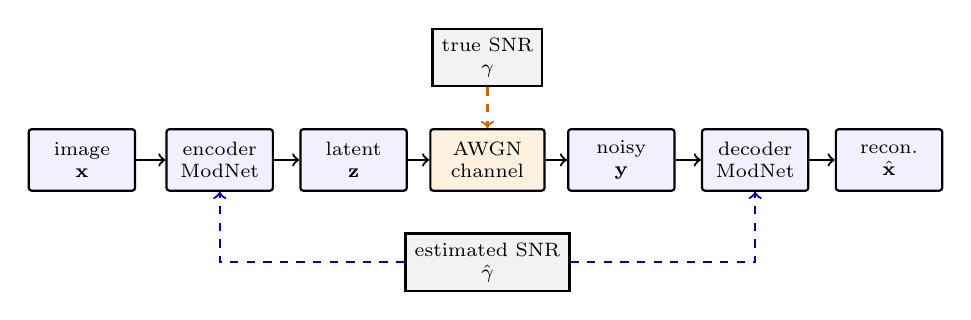
\begin{tikzpicture}[
    font=\scriptsize,
    block/.style={draw, thick, rounded corners=1pt, align=center, minimum height=0.78cm, minimum width=1.35cm, fill=blue!6},
    channel/.style={draw, thick, rounded corners=1pt, align=center, minimum height=0.78cm, minimum width=1.45cm, fill=orange!12},
    snr/.style={draw, thick, align=center, minimum height=0.5cm, minimum width=1.0cm, fill=gray!10},
    arr/.style={->, thick},
    snrarr/.style={->, thick, dashed}
]
\node[block] (x) at (0,0) {image\\$\mathbf{x}$};
\node[block] (enc) at (1.75,0) {encoder\\ModNet};
\node[block] (z) at (3.45,0) {latent\\$\mathbf{z}$};
\node[channel] (ch) at (5.15,0) {AWGN\\channel};
\node[block] (y) at (6.85,0) {noisy\\$\mathbf{y}$};
\node[block] (dec) at (8.55,0) {decoder\\ModNet};
\node[block] (xh) at (10.25,0) {recon.\\$\hat{\mathbf{x}}$};

\node[snr] (g) at (5.15,1.30) {true SNR\\$\gamma$};
\node[snr] (gh) at (5.15,-1.30) {estimated SNR\\$\hat{\gamma}$};

\draw[arr] (x) -- (enc);
\draw[arr] (enc) -- (z);
\draw[arr] (z) -- (ch);
\draw[arr] (ch) -- (y);
\draw[arr] (y) -- (dec);
\draw[arr] (dec) -- (xh);
\draw[snrarr, color=orange!80!black] (g) -- (ch);
\draw[snrarr, color=blue!70!black] (gh) -| (enc);
\draw[snrarr, color=blue!70!black] (gh) -| (dec);
\end{tikzpicture}%
}
\caption{SNR-mismatched SwinJSCC framework. The true SNR $\gamma$ determines the physical AWGN corruption, while the estimated SNR $\hat{\gamma}$ conditions the Channel ModNet branches in the encoder and decoder.}
\label{fig:framework}
\end{figure}


\section{Imperfect-CSI SwinJSCC}

The implementation separates the single SNR input of SwinJSCC into two roles. The true SNR $\gamma$ is used only by the physical channel layer, while the estimated SNR $\hat{\gamma}$ is passed to the encoder and decoder Channel ModNet branches. The original inference path is recovered by setting $\hat{\gamma}=\gamma$.

UA training samples
\begin{equation}
\gamma\sim\mathcal{S},\qquad
e\sim\mathcal{U}[-\Delta,\Delta],\qquad
\hat{\gamma}=\mathrm{clip}(\gamma+e,\gamma_{\min},\gamma_{\max}),
\label{eq:ua_sampling}
\end{equation}
and minimizes the empirical imperfect-CSI risk
\begin{equation}
\widehat{\mathcal{R}}_{\rm UA}(\theta)=
\frac{1}{|\mathcal{B}|}
\sum_{\mathbf{x}_i\in\mathcal{B}}
d\!\left(G_{\theta}(T_{\gamma_i}(F_{\theta}(\mathbf{x}_i,\hat{\gamma}_i,C)),\hat{\gamma}_i),\mathbf{x}_i\right).
\label{eq:ua_risk}
\end{equation}
When $\Delta=0$, this objective reduces to perfect-CSI fine-tuning. When $\Delta>0$, the model is trained over a local neighborhood of possible CSI estimates.

For stronger robustness, the code also supports $K$ estimated-SNR samples for the same true SNR. Let
\begin{equation}
\ell_k=d\!\left(G_{\theta}(T_{\gamma}(F_{\theta}(\mathbf{x},\hat{\gamma}_k,C)),\hat{\gamma}_k),\mathbf{x}\right),
\quad k=1,\ldots,K .
\label{eq:sample_loss}
\end{equation}
The robust training loss is
\begin{equation}
\mathcal{L}_{\rm rob}
=\frac{1}{K}\sum_{k=1}^{K}\ell_k
\lambda_{\rm tail}\,\mathrm{Top}_{1-\alpha}(\{\ell_k\}_{k=1}^{K})
\lambda_{\rm cons}\frac{1}{K-1}\sum_{k=2}^{K}\|\hat{\mathbf{x}}_k-\hat{\mathbf{x}}_1\|_1 ,
\label{eq:robust_loss}
\end{equation}
where $\mathrm{Top}_{1-\alpha}(\cdot)$ averages the largest sampled losses and the last term discourages reconstruction drift under different estimated SNR inputs.

This objective should not be interpreted as a proof of uniform improvement at every SNR pair. If the reconstruction map and distortion are locally Lipschitz with respect to $e$, then for some $K_{\theta}$,
\begin{equation}
\left|d(H_{\theta}(\mathbf{x},\gamma,e),\mathbf{x})
-d(H_{\theta}(\mathbf{x},\gamma,0),\mathbf{x})\right|
\le K_{\theta}|e|,
\label{eq:lipschitz}
\end{equation}
where $H_{\theta}$ is the full encoder-channel-decoder map under error $e$. This only justifies the distributional alignment of UA training with imperfect-CSI deployment; pointwise gains must be established empirically.

\section{Experimental Results}

The evaluation uses CIFAR10 over AWGN with $C=32$ and $\mathcal{S}=\{1,4,7,10,13\}$ dB. The baseline is the original SwinJSCC \texttt{w/SA} CIFAR10/AWGN/C32 checkpoint. All imperfect-CSI variants use the same architecture and initialize from the original checkpoint. UA uses $\Delta=3$ dB, $\gamma_{\min}=1$ dB, and $\gamma_{\max}=13$ dB. Tail-UA and Cons-UA use $K=3$ sampled estimated SNRs; Tail-UA uses $\alpha=0.8$ and $\lambda_{\rm tail}=0.5$, Cons-UA uses $\lambda_{\rm cons}=0.1$, and Tail+Cons-UA combines both terms. Training uses batch size 256, Adam optimizer, learning rate $10^{-4}$, and seed 42.

The reported metrics are PSNR and MS-SSIM(dB):
\begin{equation}
\mathrm{PSNR}=10\log_{10}\frac{255^2}{\mathrm{MSE}},
\label{eq:psnr}
\end{equation}
\begin{equation}
\mathrm{MS\text{-}SSIM}_{\rm dB}
=-10\log_{10}(1-\mathrm{MS\text{-}SSIM}).
\label{eq:msssimdb}
\end{equation}
For a mismatch matrix $\mathbf{P}_{i,j}=\mathrm{PSNR}(\gamma_i,\hat{\gamma}_j)$, diagonal entries measure matched-CSI performance and off-diagonal entries measure imperfect-CSI robustness:
\begin{equation}
\overline{P}_{\rm off}=
\frac{1}{N(N-1)}\sum_{i\ne j}\mathbf{P}_{i,j}.
\label{eq:offdiag}
\end{equation}

% Auto-generated by latex/generate_figures.py
\begin{figure*}[t]
\centering
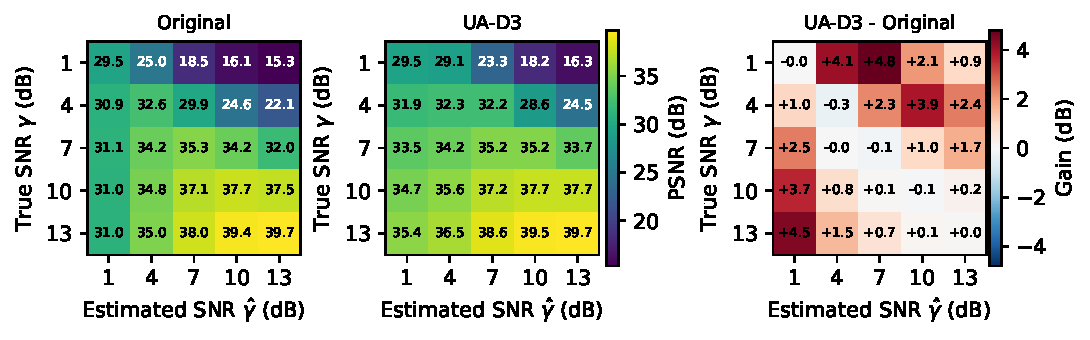
\includegraphics[width=\textwidth]{figures/fig2_psnr_heatmaps}
\caption{PSNR mismatch heatmaps on CIFAR10/AWGN/C=32. Rows denote the true physical SNR $\gamma$, columns denote the estimated modulation SNR $\hat{\gamma}$, and entries are in dB. The right panel reports the cell-wise UA-Delta3 gain over the original SwinJSCC checkpoint.}
\label{fig:psnr-heatmaps}
\end{figure*}


Fig.~\ref{fig:psnr-heatmaps} shows that the original checkpoint is sensitive to SNR mismatch, especially when a poor physical channel is overestimated. UA-Delta3 improves most off-diagonal regions. The aggregate results in Table~\ref{tab:aggregate} show the same trend: UA-Delta3 improves off-diagonal PSNR from \OrigOffPSNR{} dB to \UAOffPSNR{} dB, a gain of \GainOffPSNR{} dB, while the matched-SNR average changes by only \GainDiagPSNR{} dB.

\begin{table*}[t]
\caption{Aggregate mismatch performance on CIFAR10/AWGN/C=32. Diagonal values correspond to $\gamma=\hat{\gamma}$, off-diagonal values correspond to $\gamma\ne\hat{\gamma}$, and worst values are the minimum over the full $5\times5$ mismatch matrix.}
\label{tab:aggregate}
\centering
\scriptsize
\begin{tabular}{lrrrrrr}
\toprule
Method & Matched PSNR & Off-diag. PSNR & Worst PSNR & Matched MS-SSIM(dB) & Off-diag. MS-SSIM(dB) & Worst MS-SSIM(dB)\\
\midrule
% Auto-generated by latex/generate_figures.py
Original & \textbf{34.9688} & 29.8782 & 15.3260 & \textbf{21.1372} & 15.9684 & 3.0828 \\
UA-Delta3 & 34.8771 & \textbf{31.7947} & 16.2755 & 21.0281 & \textbf{17.9652} & 3.7445 \\
Tail-UA & 34.9254 & 31.7061 & 16.2955 & 21.0771 & 17.8702 & 3.8342 \\
Cons-UA & 34.9491 & 31.7757 & 16.2460 & 21.0971 & 17.9320 & 3.7144 \\
Tail+Cons-UA & 34.9188 & 31.7308 & \textbf{16.3152} & 21.0657 & 17.9020 & \textbf{3.8359} \\

\bottomrule
\end{tabular}
\end{table*}

\begin{table}[t]
\caption{Gains over the original checkpoint.}
\label{tab:gains}
\centering
\scriptsize
\begin{tabular}{lrrrr}
\toprule
Method & Off. PSNR & Worst PSNR & Off. MS-dB & Worst MS-dB\\
\midrule
% Auto-generated by latex/generate_figures.py
UA-Delta3 & +1.9164 & +0.9495 & +1.9969 & +0.6616 \\
Tail-UA & +1.8279 & +0.9696 & +1.9018 & +0.7513 \\
Cons-UA & +1.8974 & +0.9200 & +1.9636 & +0.6316 \\
Tail+Cons-UA & +1.8526 & +0.9892 & +1.9336 & +0.7530 \\

\bottomrule
\end{tabular}
\end{table}

The variants show different robustness trade-offs. UA-Delta3 gives the strongest average off-diagonal result, improving off-diagonal MS-SSIM(dB) by \GainOffMSSSIM{} dB. Cons-UA preserves the matched-SNR diagonal best among the imperfect-CSI variants, consistent with its reconstruction-stability penalty. Tail+Cons-UA gives the best worst-case robustness, improving worst-case PSNR by \TailConsWorstPSNRGain{} dB and worst-case MS-SSIM(dB) by \TailConsWorstMSSSIMGain{} dB over the original checkpoint. These results support using UA as the main method and treating tail/consistency losses as robustness-oriented ablations rather than uniformly superior replacements.

% Auto-generated by latex/generate_figures.py
\begin{figure*}[t]
\centering
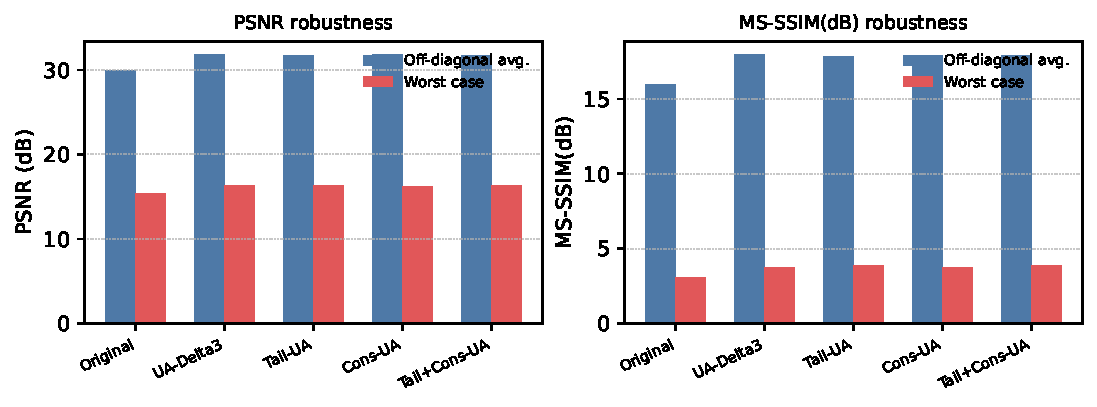
\includegraphics[width=\textwidth]{figures/fig3_aggregate_bars}
\caption{Aggregate robustness comparison across the original checkpoint and imperfect-CSI training variants. Off-diagonal averages characterize average mismatch robustness, while worst-case values characterize the weakest SNR pair in the matrix.}
\label{fig:aggregate-bars}
\end{figure*}

% Auto-generated by latex/generate_figures.py
\begin{figure*}[t]
\centering
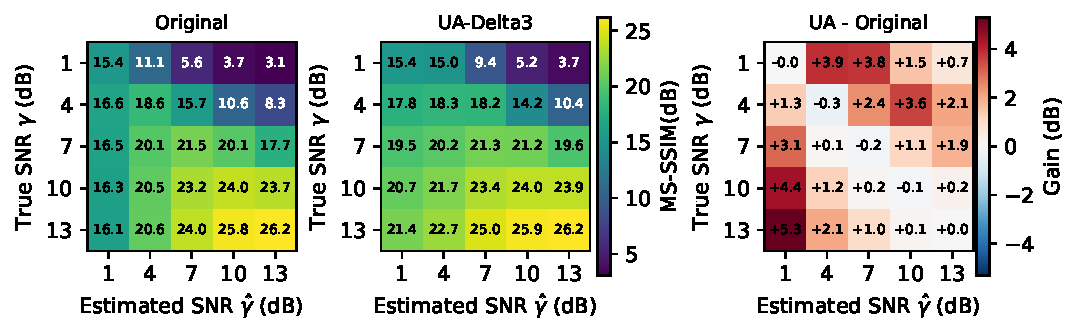
\includegraphics[width=\textwidth]{figures/fig4_msssim_heatmaps}
\caption{MS-SSIM(dB) mismatch heatmaps on CIFAR10/AWGN/C=32. The pattern is consistent with PSNR: UA-Delta3 improves most off-diagonal regions while slightly reducing the matched-SNR diagonal average.}
\label{fig:msssim-heatmaps}
\end{figure*}


Table~\ref{tab:cases} lists the largest UA-Delta3 PSNR gains. The most prominent case is $\gamma=1$ dB and $\hat{\gamma}=7$ dB, where PSNR improves by 4.7989 dB. This is a practically important mismatch direction: the modulation network is conditioned on an overoptimistic SNR while the physical channel is poor.

\begin{table}[t]
\caption{Representative off-diagonal PSNR gains of UA-Delta3.}
\label{tab:cases}
\centering
\scriptsize
\begin{tabular}{rrrrr}
\toprule
$\gamma$ & $\hat{\gamma}$ & Original & UA & Gain\\
\midrule
% Auto-generated by latex/generate_figures.py
1 & 7 & 18.5161 & 23.3151 & +4.7989 \\
13 & 1 & 30.9903 & 35.4478 & +4.4575 \\
1 & 4 & 24.9906 & 29.1104 & +4.1198 \\
4 & 10 & 24.6440 & 28.5768 & +3.9328 \\
10 & 1 & 31.0376 & 34.7060 & +3.6684 \\

\bottomrule
\end{tabular}
\end{table}

The current evidence is intentionally bounded. It establishes the mismatch behavior on CIFAR10/AWGN/C=32 and one random seed. Rayleigh fading, high-resolution images, multiple CBR settings, repeated seeds, and $\Delta$ ablations remain necessary before making broader deployment claims.

\section{Conclusion}

This letter reformulates adaptive SwinJSCC for imperfect CSI by separating the physical SNR from the estimated SNR used by Channel ModNet. The resulting UA training objective aligns the optimization distribution with bounded SNR estimation errors. On CIFAR10/AWGN/C=32, UA-Delta3 yields a 1.9164 dB off-diagonal PSNR gain with only a 0.0917 dB matched-SNR PSNR reduction, while tail-risk and consistency variants improve complementary robustness measures. Future work will extend the evaluation to fading channels, rate adaptation, high-resolution data, and repeated-seed uncertainty analysis.

\bibliographystyle{IEEEtran}
\bibliography{references}

\end{document}
